\documentclass{beamer}

\usetheme{CambridgeUS}
\usecolortheme{dolphin}

\usepackage{graphicx}

\title{Visualizing Graduate Admissions Data}

\author{Aaron Doubek-Kraft, adoubekk@ucsc.edu}

\date{March 6, 2017}

\begin{document}
	
	\frame{\titlepage}
	
	\begin{frame}{Problem}
		\begin{itemize}
			\item Given the unusually large applicant pool to the UCSC Computer Science graduate program, determine if any correlation exists between:
			\begin{itemize} \item an applicant's quantitative records (GPA, test scores, etc.) 
							\item their potential to succeed in the program
							\item their strength/interest in a given research area
			\end{itemize}
			\item Create a tool to visualize general multivariate datasets
		\end{itemize}	
	\end{frame}
	
	\begin{frame}{Approach}
		\begin{itemize}
			\item Parallel Coordinate Plots: Sets of parallel axes connected by polylines that represent an individual record
			\item Strengths
			\begin{itemize}
				\item Standard and generic approach to multivariate visualization
				\item Easy to identify trends in the data
				\item Straightforward implementation
			\end{itemize}
			\item Weakness
			\begin{itemize}
				\item Quickly becomes visually cluttered for large datasets
			\end{itemize}
			\item Improving Readability
			\begin{itemize}
				\item Map polyline color to group membership
				\item Highlight group or subset by hiding or graying out other lines
				\item Highlight data that falls within a particular range on an axis (brushing)
			\end{itemize}
		\end{itemize}
	
	\end{frame}
	
	\begin{frame}{Implementation}
		\begin{itemize}
			\item Operations on dataset: Python scripts
			\begin{itemize}
				\item Normalize test scores
				\item Strip rankings from research interests to improve grouping
			\end{itemize}
			\item Visualization: Web Application
			\begin{itemize}
				\item d3.js: Graphics
				\item jQuery: DOM Manipulation
				\item w3.css: Style Framework
			\end{itemize}
		\end{itemize}
	\end{frame}
	
	\begin{frame}{Results}
		\begin{figure}[h]
			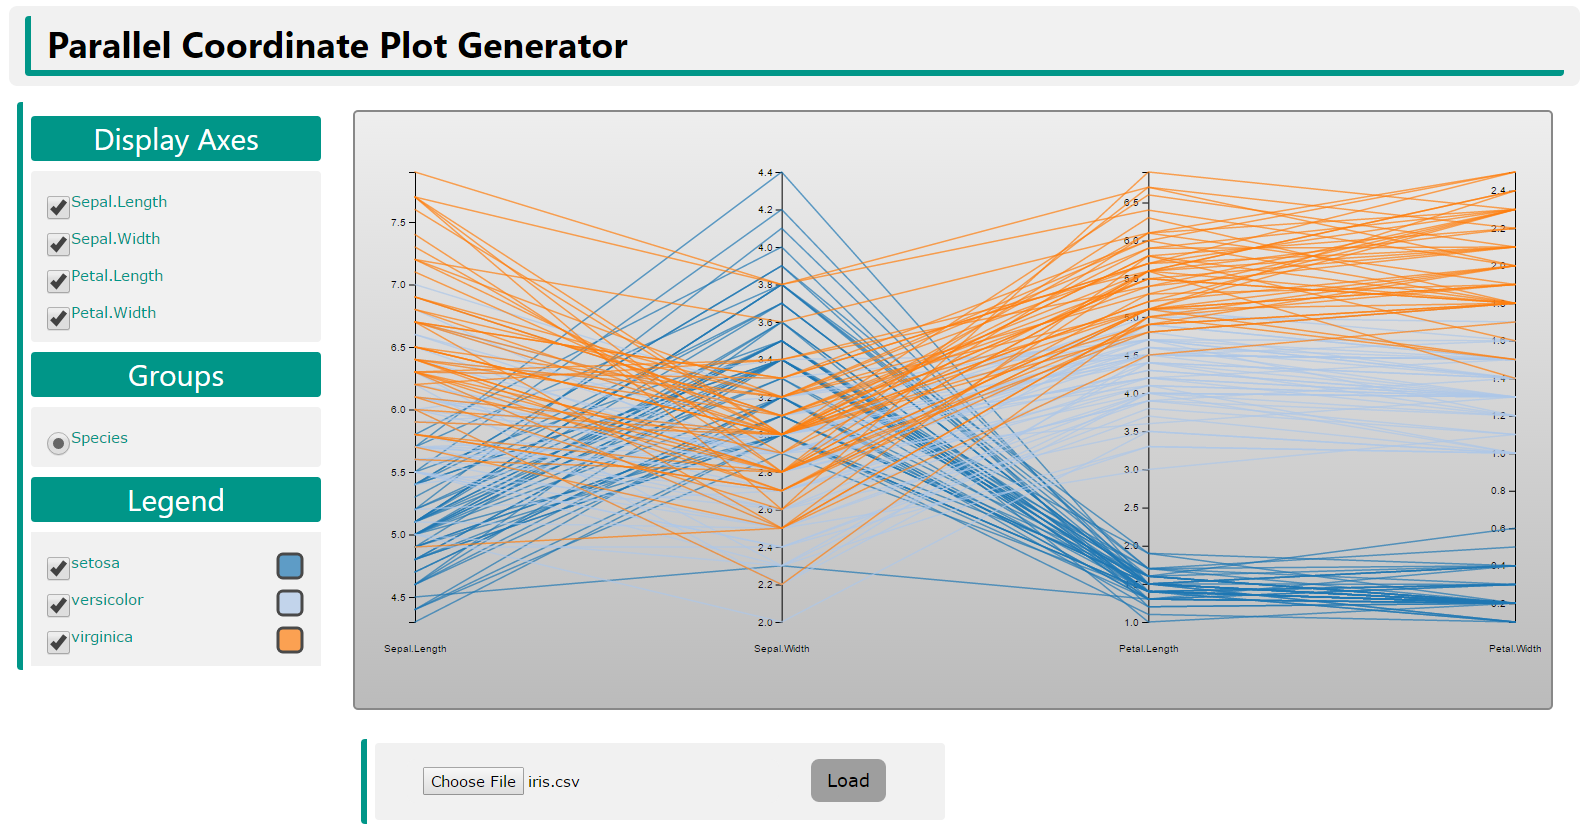
\includegraphics[width=\linewidth]{results.png}
			\caption{Visualizing Edgar Anderson's Iris dataset}
			\label{fig:Result}
		\end{figure}		
	\end{frame}
	
	\begin{frame}{To Complete}
		\begin{itemize}
			\item Processing and analysis of graduate admissions dataset
			\item Additional user interactions, such as brushing
			\item User customization of appearance of visualization
		\end{itemize}
	\end{frame}

\end{document}
